Eine \mZbO\ schwere Zugbrücke wird von einem Seil festgehalten, welches in der Mitte der Brücke angreift. Die Zugkraft des Seils beträgt \FSzO. Unter welchem Winkel greift das Seil an der Brücke an? Bestimmen Sie Betrag und Richtung der Kraft im Drehpunkt D.

\begin{center}
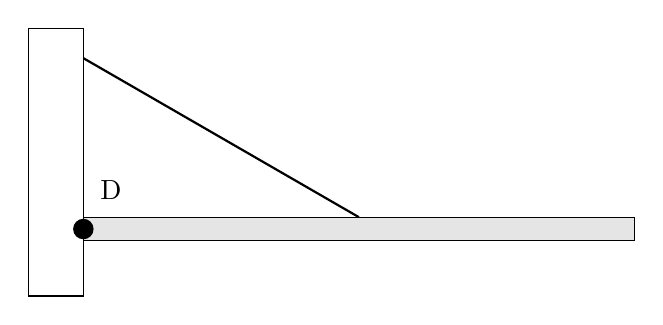
\begin{tikzpicture}
 \draw (-0.7,-1.0) rectangle (0,2.4);
 \fill[gray!20] (0,-0.3) rectangle (7,0);
 \draw (0,-0.3) rectangle (7,0);
 \draw[thick] (0,2.02) -- (3.5,0);
 \fill (0,-0.15) circle (0.13);
 \node at (0.35,0.35) {D};
\end{tikzpicture}
\end{center}
